\documentclass[notitlepage]{article}
\ifdefined\HCode
  \def\pgfsysdriver{pgfsys-dvisvgm4ht.def} % for HTML output
\fi
\usepackage[a4paper,margin=2cm]{geometry}
\usepackage[T1]{fontenc}
\ifx\HCode\undefined
\usepackage{beton}
\usepackage{eulervm}
\fi
\setlength{\parindent}{0pt}
\setlength{\parskip}{1ex}
\usepackage{listings}
\usepackage{hyperref}
\usepackage{amsmath,amssymb,siunitx}
\usepackage[x11names,svgnames]{xcolor}
\usepackage{tikz}
\usetikzlibrary{arrows,backgrounds,calc,patterns}

\usepackage{imakeidx}
\makeindex[columns=1,title=Alphabetical Index,intoc]

% Font substitution: taken from https://ctan.org/tex-archive/macros/latex/contrib/beton/beton.pdf
\ifx\HCode\undefined
\AtBeginDocument{
  \DeclareFontShape\encodingdefault{ccr}{bx}{n}{<->sub*cmss/sbc/n}{}
  \DeclareFontShape\encodingdefault{ccr}{bx}{it}{<->sub*cmss/sbc/it}{}
  \DeclareFontShape\encodingdefault{ccr}{bx}{sl}{<->sub*cmss/sbc/sl}{}
  \DeclareFontShape\encodingdefault{ccr}{bx}{sc}{<->sub*cmss/sbc/sc}{}
}
\fi

\lstdefinestyle{luastyle}{
  language=[5.1]Lua,
  basicstyle=\ttfamily,
  columns=spaceflexible,
  tabsize=2
}

\ifdefined\HCode
\newcommand{\var}[1]{$\langle$\texttt{#1}$\rangle$}
\newcommand{\varnth}[2]{\var{#1\HCode{<sub>}#2\HCode{</sub>}}}
\newcommand{\ovar}[1]{$[\langle$\texttt{#1}$\rangle]$}
\else
\newcommand{\var}[1]{$\mathit{\langle}$\textrm{\textmd{\textit{#1}}}$\mathit{\rangle}$}
\newcommand{\varnth}[2]{\var{#1$_{#2}$}}
\newcommand{\ovar}[1]{$\mathit{[\langle}$\textrm{\textmd{\textit{#1}}}$\mathit{\rangle]}$}
\fi

\newcommand{\vari}[1]{\varnth{#1}{1}}
\newcommand{\varii}[1]{\varnth{#1}{2}}

\def\luatrue{\texttt{true}}
\def\luafalse{\texttt{false}}
\def\luanil{\texttt{nil}}
\def\advtrains{\textsc{advtrains}}

\newenvironment{centeredtikzpicture}[1][]{
  \begin{center}
    \begin{tikzpicture}[#1]
    }{
    \end{tikzpicture}
  \end{center}
}

\newenvironment{apidoc}[1]{
  \begin{list}{}{
  \setlength{\labelwidth}{0pt}
  \setlength{\labelsep}{0pt}
  \setlength{\leftmargin}{0pt}
  \setlength{\listparindent}{1em}
}
\index{#1}
\ifdefined\HCode
\providecommand{\apientp}[2]{\HCode{<br/>}##1\HCode{<span style="float:right">}##2\HCode{</span><br/>}}
\else
\providecommand{\apientp}[2]{##1\hfill {##2}\par}
\fi
\providecommand{\apient}[2]{\apientp{##1}{##2}\index{##1}}
\providecommand{\apip}[2]{\apientp{\texttt{##1}}{##2}}
\providecommand{\api}[2]{\apient{\texttt{##1}}{##2}}
\providecommand{\apiasp}[1]{\apient{##1}{signal aspect}}
\providecommand{\apicmd}[1]{\api{##1}{command}}
\providecommand{\apienum}[1]{\apip{##1}{enumeration}}
\providecommand{\apifield}[1]{\apip{##1}{field}}
\providecommand{\apiitem}[1]{\apient{##1}{item}}
\providecommand{\apivar}[1]{\apip{##1}{variable}\index{#1!\texttt{##1}}}
\providecommand{\apifunc}[2]{\apip{##1(##2)}{function}\index{#1!\texttt{##1}}}
\providecommand{\apilex}[1]{\apip{##1}{lexical syntax}}
\providecommand{\apipat}[1]{\apip{##1}{pattern}}
\providecommand{\apiterm}[1]{\apient{##1}{term}}
\providecommand{\apitrainmode}[1]{\apient{##1}{train mode}}
\providecommand{\apiui}[1]{\apientp{##1}{UI element}}
}{\end{list}}

\tikzset{
  signal/.pic = {
    \draw (0,0) -- (0,0.2) -- (0.15,0.2);
    \draw [fill=#1] (0.15,0.2) circle [radius=0.05];
  },
  tcb/.pic = {
    \draw (0,0) -- (0,0.2);
    \draw [<->] (-0.15,0.2) -- (0.15,0.2);
  }
}
\ifdefined\HCode
\tikzset{
  pattern or line fill/.style={fill=cyan}
}
\else
\tikzset{
  pattern or line fill/.style={pattern=north west lines,pattern color=gray}
}
\fi

\title{The \advtrains{} mod for Minetest}
\author{}

\begin{document}

\ifx\HCode\undefined
\thispagestyle{empty}
\begin{tikzpicture}[remember picture,overlay]
  \newcommand{\HUGE}[1]{\scalebox{2}{\Huge #1}}
  \fill[Turquoise] (current page.south west) rectangle (current page.north east);
  \node [below,inner sep=0,outer sep=0,name=coverimage] at (current page.north) {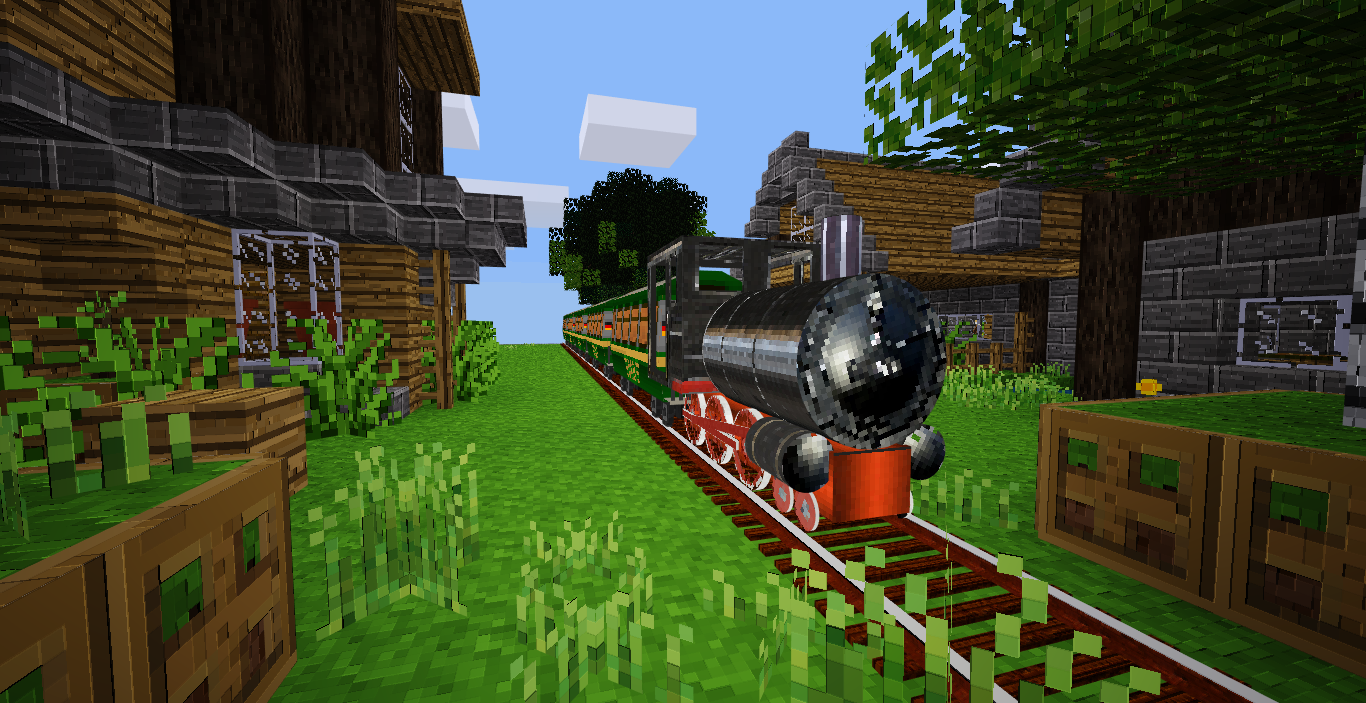
\includegraphics[width=2\paperwidth]{../../screenshot.png}};
  \draw ($0.5*(coverimage.south)+0.5*(current page.south)$)
  +(0,0.5) node [above] {\HUGE{Advanced Trains}}
  +(0,-0.5) node [below] {\HUGE{for Minetest}};
\end{tikzpicture}
\fi

\newpage
\maketitle
\tableofcontents

\newpage
\section*{Introduction}
\addcontentsline{toc}{section}{Introduction}
\advtrains{} is a mod with the goal of introducing realistic trains and rail equipments. It also has features allowing automated trains on a large scale, including interlocking and a few methods of scripting.

This manual is written for the specific version of \advtrains{} that the corresponding \LaTeX{} source is distributed with. It is divided into two parts, where the first part mainly documents the various features of \advtrains, and the second part focuses on the internals of \advtrains.

\subsection*{Acknowledgments}

A notable portion of the manual is influenced by various other guides and manuals for \advtrains. In particular:
\begin{itemize}
\item The format of the API documentation is influenced by R$^7$RS.
\item Section \ref{s:interlocking} is written with reference to orwell's interlocking guide and Blockhead's video explaining the three-station setup. The links to both sources can be found in that section.
\item Section \ref{s:luaatc} is a reformatted and restructured version of the LuaATC documentation, written by orwell and Maverick2797.
\item Section \ref{s:tilrwt} is a modified version of the railway time API documentation written by orwell. Part of the section is also taken from \texttt{advtrains\_line\_automation/railwaytime.lua}
\end{itemize}

\subsection*{Conventions}
\begin{itemize}
\item Unless otherwise specified, the unit of length is meter (or, more technically, nodes).
\item Unless otherwise specified, the unit of speed is meter per second.
\item Unless otherwise specified, the unit of acceleration is meter per second squared.
\item The \tikz \pic at (0,0) {tcb}; symbol stands for a TCB assigned to the track.
\item The \tikz \pic (0,0) {signal=red}; symbol stands for a TCB assigned to the track with a signal assigned to the TCB side opposite of that of the direction in which the TCB is facing (here: the signal is assigned to the left side of the TCB).
\item Arguments to functions and ATC commands are delimited using angle brackets \var{like this}.
\item Argument names are generally lowercase, but the first letter may be capitalized.
\item Lua string constants are written without quotation marks when the content does not resemble any numeric or symbolic constant and when used as enumerators or table indices.
\item Like in other parts of \advtrains, Lua code is indented with tabs.
\item An error situation that may or may not be reported are referred to as \textit{an error}. An error situation that is always reported is one where \textit{an error is signaled}.
\item Unless otherwise specified, the return value of any Lua API function is undefined.
\item The action of left-clicking a node with a trackworker is called \textit{rotation}. The action of right-clicking a node with a trackworker is called \textit{adjustment}.
\end{itemize}

\newpage
\part{User Guide}

\section{Tracks}

\subsection{Angles}

Unlike regular carts in Minetest, tracks can connect in 16 cardinal directions instead of four:

\begin{centeredtikzpicture}
  \draw[step=1,gray,very thin] (0,0) grid (5,5);
  \def\dirs{
    0/1,1/2,1/1,2/1,1/0,2/-1,1/-1,1/-2,
    0/-1,-1/-2,-1/-1,-2/-1,-1/0,-2/1,-1/1,-1/2
  }
  \foreach \dx/\dy in \dirs {
    \draw[pattern or line fill,shift={(\dx,\dy)}] (2,2) rectangle +(1,1);
  }
  \foreach \dx/\dy in \dirs {
    \draw[very thick,->] (2.5,2.5) -- +(\dx,\dy);
  }
  \node[circle,draw=black,fill=white,text=black] at (2.5,2.5) {A};
\end{centeredtikzpicture}

In the figure above, the filled squares show possible connections from the track at A.

Tracks that are not axis-aligned are sometimes referred to as 30\textdegree{} (although it is technically $\arcsin 0.5$) or 45\textdegree{} tracks. However, the specific meaning of the terms may depend on the context of the discussion.

The use of 16 cardinal directions instead of four allows the creation of curves that are more realistic than their counterparts made using minecart rails. A typical 90\textdegree{} curve looks like this:

\begin{centeredtikzpicture}
  \draw[step=1,gray,very thin] (0,0) grid (6,6);
  \foreach \x/\y in {0/0,0/1,1/3,2/4,4/5,5/5} {
    \draw[pattern or line fill] (\x,\y) rectangle +(1,1);
  }
  \draw[<->,very thick] (0.5,0.5) -- ++(0,1) -- ++(1,2) -- ++(1,1) -- ++(2,1) -- ++(1,0);
\end{centeredtikzpicture}

However, this is still notably smaller than in real life. For comparison, the smallest curve for the H0 model (1:87) has a radius of 360mm, which is 31.32m when scaled to real life.

\subsection{Track placement}

The usual way of placing a track is with a ``track placer'', a tool that places the tracks and, in many cases, automatically adjusts them to connect to nearby tracks.

You can get track placers from the creative inventory or by crafting. Please refer to the crafting guide for the recipe.

To place the track, simply right click the node to place the track on with the trace placer. To place slopes, face the upper end of the slope and click on the $n$th node before the upper end of the slope for a slope with an incline of $1/n$. For example, if you want to build a slope with an incline of 50\% (the slope marked gray), you would look at node A and click on node B while standing in such a way that the direction you are looking at is also the direction in which the slope goes up (e.g. at node P):
\begin{centeredtikzpicture}
  \draw[step=1,gray!50!white,thin] (-2,0) grid (3,2);
  \draw[fill=black!40!gray] (0,1) -- ++(2,0) -- ++(0,1) -- cycle;
  \foreach \x/\y/\l in {0/0/B,1/0/,2/1/A}{
    \draw[fill=cyan] (\x,\y) rectangle +(1,1);
    \node[text=black,shift={(0.5,0.5)}] at (\x,\y) {\l};
  }
  \node[text=black] at (-1.5,1.5) {P};
\end{centeredtikzpicture}

Please note that, in the figure above, the three colored nodes must already be placed.

\subsection{Track adjustment}
You can use a trackworker to make certain adjustments to tracks. Specifically,
\begin{itemize}
\item Left-clicking on a track with the trackworker toggles between the variants of the particular track, if any.
\item Right-clicking on a track with the trackworker rotates the track counterclockwise.
\end{itemize}

Typical examples of ``variants'' of tracks include turnouts and curves. Please note that Y-turnouts and different types of crossings have their own variants. These variants are described below. Additionally, special tracks (ATC track, station tracks, etc.) are usually only straight, and certain mods that provide additional tracks (e.g. linetrack) may not provide a full set of tracks available in the official track set.

\subsection{Turnouts}
Turnouts are tracks that connect tracks from more than one direction. Some examples of turnouts are shown below.

\begin{centeredtikzpicture}
  \draw[step=1,gray,thin,shift={(-0.5,-0.5)}] (0,0) grid (10,4);
  \def\turnouts{
    1/{0/-1, 0/1, -1/2},
    2/{0/-1, 0/1, 1/2},
    5/{0/-1, -1/2, 1/2},
    8/{0/-1, 0/1, -1/2, 1/2},
  }
  \foreach \base/\dirs in \turnouts {
    \draw[->, very thick] (\base,1) -- +(0,-1);
    \foreach \dx/\dy in \dirs {
      \draw[->, very thick] (\base,1) -- +(\dx,\dy);
    }
  }
\end{centeredtikzpicture}

The figure above aligns the tracks in a way that they always merge into the track that connects to the south. This is mainly done for intuitivity - you can rotate the turnouts freely in any of the 16 directions.

\subsection{Crossings}\label{s:xings}
There are a few crossing nodes that allow you to create intersections:
\begin{itemize}
\item Perpendicular crossings: intersections where two tracks are perpendicular to each other
\item $90^\circ+x$ crossings: intersections where only one of the two tracks is axis-aligned
\item diagonal crossings: other crossings that do not fit in the two categories mentioned above
\end{itemize}

Each type of crossing has its own track placer. The trackworker can not be used to switch between the different types of crossing tracks.

The figure below shows a few examples of crossings that are available.
\begin{centeredtikzpicture}[scale=0.9]
  \draw[gray,thin, shift={(-0.5,-0.5)}] (0,0) grid (11,11);
  \def\xings{
    2/2/1/2/2/1,
    2/8/2/1/1/-2,
    8/1/2/1/1/0,
    8/5/2/1/2/-1,
    8/9/2/1/1/-1
  }
  \foreach \x/\y/\ax/\ay/\bx/\by in \xings {
    \foreach \dx/\dy in {\ax/\ay,\bx/\by} {
      \draw [<->, very thick] ($(\x,\y)-(\dx,\dy)$) -- +($2*(\dx,\dy)$);
    }
  }
\end{centeredtikzpicture}

It is also possible to create track layouts without using crossings. Some examples are shown below.

\begin{centeredtikzpicture}[scale=0.9]
  \draw[gray,thin, shift={(-0.5,-0.5)}] (0,0) grid (12,4);
  \def\lines{
    0/0/3/3,0/3/3/0,
    5/0/11/3,6/3/9/0
  }
  \def\squares{
    0/0,1/1,2/2,3/3,0/3,1/2,2/1,3/0,
    5/0,7/1,9/2,11/3,6/3,7/2,8/1,9/0
  }
  \foreach \x/\y in \squares {
    \draw [pattern or line fill,shift={(-0.5,-0.5)}] (\x,\y) rectangle +(1,1);
  }
  \foreach \ax/\ay/\bx/\by in \lines {
    \draw [<->, very thick] (\ax,\ay) -- (\bx,\by);
  }
\end{centeredtikzpicture}

Exercise: Build a T junction. You will need this later in section \ref{s:iljunctions}. You can also look at the scheme in that section if you need a hint.

\subsection{Special tracks}

\advtrains{} also have a few special tracks, some of which are explain in their own sections.

\begin{apidoc}{Special tracks}
\item \apiitem{ATC track} Track that sends ATC commands to a train (see section \ref{s:atc} for more information)
\item \apiitem{Loading track} Track that makes a train load as many items as possible from a chest below the track if the train is moving in the direction indicated by the arrow on the track at a speed lower than 2m/s.
\item \apiitem{Unloading track} Track that makes a train unload as many items as possible into a chest below the track if the train is moving in the direction indicated by the arrow on the track at a speed lower than 2m/s.
\item \apiitem{Temporary speed restriction rail} Track that forces a train to pass with an arbitrary speed limit.
\item \apiitem{Station track} Track that makes trains temporarily stop at a given point (see section \ref{s:stoprail} for more information)
\item \apiitem{LuaATC track} Track that can be programmed in Lua (see section \ref{s:luaatc} for more information).
\end{apidoc}

\section{Train controls}\label{s:controls}
To get on a train, click on the train while its doors are open, or click on the train while holding the Sneak key. You need to be in the driver stand in order to control the train.

Train movement currently depends on two factors: the lever of the train and the percentage of locomotives in the train. Details on train physics can be found in section \ref{s:physics}.

Unlike in real life, levers are not moved continuously. Instead, there are a few lever ``positions'' that are recognized by \advtrains{}:

\begin{itemize}
\item The lever 0 triggers the emergency brake. It can be triggered by the ATC \texttt{BB} command (see section \ref{s:atc}).
\item The lever 1 triggers the default brake.
\item The lever 2 (``roll'') slows down a train as if it was on a horizontal surface without any traction
\item The lever 3 does not affect the speed of the train.
\item The lever 4 accelerates the train.
\end{itemize}

\subsection{Train formspec}\label{s:trainformspec}
If you have access to the driver stand of the wagon, right-clicking the train will open up a formspec will a few buttons, depending on the status of the train:
\begin{apidoc}{Train formspec}
\item \apiui{Passenger area} Move to the passenger area.
\item \apiui{Driver stand} Move to the driver stand.
\item \apiui{Onboard computer} Open the onboard computer.
\item \apiui{Wagon properties} Allow setting wagon properties.
\item \apiui{Get off} Get off the train.
\item \apiui{(Doors closed)} Get off the train by right-clicking the train while holding the Sneak key.
\end{apidoc}

\subsection{Onboard computer}\label{s:bordcom}
The onboard computer allow setting certain properties of the train. Feel free to explore it yourself. A few fields are explained here in detail:
\begin{apidoc}{Onboard computer}
\item \apiui{Line number} The line name of the train. Despite the label, you can set this to anything. This field is mainly used for interlocking.
\item \apiui{Routing code} The routing code of the train, separated by space characters. This field is mainly used for interlocking.
\item \apiui{Train overview} This section is only shown when the train is not moving. It allows you to couple and decouple wagons from the train.
\end{apidoc}

\subsection{HUD}\label{s:trainhud}

The HUD is a visual representation of certain information about the train. An overview of the HUD is as follows:

\begin{centeredtikzpicture}[xscale=0.025,yscale=-0.025]
  \footnotesize
  \newcommand{\rect}[3]{
    \draw[#1] #2 rectangle #3;
  }
  \newcommand{\frect}[3]{
    \rect{#1,fill=#1}{#2}{#3}
  }
  \newcommand{\sevenseg}[5]{
    \def\x{#2}
    \def\y{#3}
    \def\w{#4}
    \def\h{#5}
    \def\segs{
      {(\h,0)}/\w/\h,
      {(0,\h)}/\h/\w,
      {($(\w,0)+(\h,\h)$)}/\h/\w,
      {($(0,\w)+(\h,\h)$)}/\w/\h,
      {($(0,\w)+2*(0,\h)$)}/\h/\w,
      {($(\w,\w)+\h*(1,2)$)}/\h/\w,
      {($2*(0,\w)+\h*(1,2)$)}/\w/\h
    }
    \foreach \off/\sx/\sy in \segs {
      \frect{#1}{(\x,\y) ++\off}{++(\sx,\sy)};
    }
  }
  \newcommand{\filledcirclelabel}[2]{
    \node[circle,text=black,fill=white,draw=black] at #1 {#2};
  }
  \newcommand{\plainlabel}[2]{
    \node[text=black] at #1 {#2};
  }
  \frect{black}{(0,0)}{+(440,110)}
  \frect{cyan}{(10,10)}{++(30,30)}
  \plainlabel{(25,25)}{1}
  \frect{red}{(50,10)}{++(30,30)}
  \plainlabel{(65,25)}{2}
  \frect{orange}{(90,10)}{++(30,30)}
  \plainlabel{(105,25)}{3}
  \frect{orange}{(130,10)}{++(30,5)}
  \frect{orange}{(130,35)}{++(30,5)}
  \foreach \i in {130,141,152}{\sevenseg{orange}{\i}{18}{4}{2}}
  \filledcirclelabel{(145,25)}{4}
  \frect{white}{(187,10)}{++(26,30)}
  \frect{black}{(189,12)}{++(22,11)}
  \frect{white}{(170,10)}{++(15,30)}
  \frect{black}{(172,12)}{++(11,11)}
  \frect{white}{(215,10)}{++(15,30)}
  \frect{black}{(217,12)}{++(11,11)}
  \filledcirclelabel{(200,25)}{5}
  \draw[cyan,fill=cyan] (245,10)++(0,15) -- +(15,0) -- +(7.5,-15);
  \draw[orange,fill=orange] (245,85) -- +(15,0) -- +(7.5,15);
  \frect{DarkSlateGray}{(250,35)}{++(5,40)}
  \filledcirclelabel{(252.5,55)}{6}
  \frect{cyan}{(275,10)}{++(5,18)}
  \frect{white}{(275,28)}{++(5,18)}
  \frect{orange}{(275,46)}{++(5,36)}
  \frect{red}{(275,82)}{++(5,18)}
  \frect{DarkSlateGray}{(292,16)}{++(6,78)}
  \filledcirclelabel{(295,55)}{7}
  \foreach \x in {10,21,...,120}{\frect{white}{(\x,65)}{++(8,20)}}
  \filledcirclelabel{(69,75)}{8}
  \foreach \x in {197,208,219}{\frect{DarkSlateGray}{(\x,65)}{++(8,20)}}
  \filledcirclelabel{(212,75)}{9}
  \frect{red}{(183,60)}{++(3,30)}
  \filledcirclelabel{(184.5,75)}{10}
  \draw[red,fill=red] (133,50) -- +(15,0) -- +(7.5,15);
  \plainlabel{(140.5,54)}{4}
  \draw[cyan,fill=cyan] (89,100) -- +(15,0) -- +(7.5,-15);
  \plainlabel{(96.5,96)}{11}
  \sevenseg{red}{320}{10}{30}{10}
  \sevenseg{red}{380}{10}{30}{10}
  \filledcirclelabel{(375,55)}{8}
\end{centeredtikzpicture}

\begin{enumerate}
\item ATC indicator
\item LZB indicator
\item Shunt indicator
\item Aspect of and distance to the upcoming LZB entry (usually a signal)
\item Door indicator
\item Reverser
\item Lever
\item Speed indicator
\item Max speed indicator
\item Speed restriction indicator
\item ATC target speed indicator
\end{enumerate}

\subsection{Keybindings}\label{s:keybindings}
Hitting any movement key as a passenger will drop you off the train when a door is open or when the wagon has no doors. Alternatively, the Sneak+Aux1 keystroke will drop you off a train, regardless of whether doors are open.

The following keybindings are available to the driver, regardless of the mode of the train.
\begin{itemize}
\item Sneak+Forward: Set the ATC target speed to the maximum speed
\item Sneak+Backward: Set the ATC target speed to 0
\item Sneak+Left: Set the ATC target speed to 4
\item Sneak+Right: Set the ATC target speed to 8
\item Sneak+Jump: Open the onboard computer
\item Jump+Backward: Emergency brake
\end{itemize}

\subsection{Manual control}\label{s:manual-control}
Manual control makes the user in charge controlling the train. The following keybindings are available when manually controlling the train:
\begin{itemize}
\item Forward: Accelerate.
\item Backward: Roll when the train is moving, reverse otherwise.
\item Left: Open/Close the door on the left side and, if the door on the right side is open, close the door on the right side.
\item Right: Open/Close the door on the right side and, if the door on the left side is open, close the door on the left side.
\item Jump: Brake or, in ATC mode, switch to manual control
\end{itemize}

These keybindings (except for the jump key) do not work in ATC mode. The lever is moved to a specific level only as long as the corresponding key is pressed.

\subsection{ATC}\label{s:atc}

ATC is a method of automatically controlling trains. Certain modes can be directly activated using specific keybindings, but more common ways of using ATC include:
\begin{itemize}
\item Directly using ATC tracks,
\item Using station/stop tracks, and
\item Using LuaATC
\end{itemize}

ATC tracks can be used to send custom ATC commands to the train passing the track. The ATC commands available are listed below:

\begin{apidoc}{ATC}
\item \apilex{A0} Disables ARS.
\item \apilex{A1} Enables ARS.
\item \apilex{BB} Actives the emergency brake until the train stops.
\item \apilex{B\var{speed}} Brakes until \var{speed} is reached.
\item \apilex{Cpl} Enables autocouple mode.
\item \apilex{D\var{time}} Waits for \var{time} seconds before continuing execution.
\item \apilex{I\var{condition}\var{consequent};} Executes \var{consequent} if \var{condition} is met.
\item \apilex{I\var{condition}\var{consequent}E\var{alternate};} Executes \var{consequent} if \var{condition} is met, \var{alternate} otherwise.
\item \apilex{K} Kicks all passengers (players not driving the train) off the train only when the train is stopped and its doors are open.
\item \apilex{OC} Closes doors on both sides.
\item \apilex{OL} Opens doors on the left side and closes doors on the right side (if open).
\item \apilex{OR} Opens doors on the right side and closes doors on the left side (if open).
\item \apilex{R} Reverses the train only when the train is not moving.
\item \apilex{S\var{speed}} Accelerates to \var{speed} or roll if the train is faster then \var{speed}.
\item \apilex{W} Waits until the target set by \texttt{S} or \texttt{B} command is reached.
\end{apidoc}

For the \texttt{B}, \texttt{D}, and \texttt{S} commands, the argument should be written immediately after the command, without any whitespace.

The following \var{condition}s are available for the ATC \texttt{I} command:

\begin{apidoc}{ATC conditions}
\item \apilex{+} True when the train is driving in the same direction as the arrows on the ATC rail.
\item \apilex{-} True when the train is driving in the opposite direction of the arrow on the ATC rail.
\item \apilex{<\var{speed}} True when the train is slower than \var{speed}.
\item \apilex{>\var{speed}} True when the train is faster than \var{speed}.
\item \apilex{<=\var{speed}} True when the train is not faster than \var{speed}.
\item \apilex{>=\var{speed}} True when the train is not slower than \var{speed}.
\end{apidoc}

\subsection{LZB}\label{s:lzb}

\fbox{\parbox{\textwidth}{The explanation of LZB is specific to \advtrains. Please refer to other sources, such as Wikipedia, for information on the use of LZB in real-life rail lines.}}

In \advtrains, LZB is a system that makes sure that trains realistically brake to the desired speed, overriding ATC and manual control if necessary.

LZB speed targets are temporary and associated to a specific point - it only makes sure that the front part of the train passes that point at the desired speed. For example, a point speed restriction rail with a speed target of 3 will only make sure that the front of the train passes the PSR rail at the speed of 3, but the train is allowed to accelerate up to the speed limit (or the maximum speed, if there is no speed limit) after the head of the train passes the PSR rail.

\subsection{Minor modes}\label{s:trainminormodes}
The modes described here do not override any of the modes described above, but rather coexist with these.

\begin{apidoc}{Train modes}{}
\item \apitrainmode{ARS} If enabled, signals using ARS will select the appropriate route for the train. If ARS is disabled for the train, signals using ARS will not select any route for the train. This mode is enabled by default.
\item \apitrainmode{Autocouple mode} If enabled, the train will automatically couple with any train it collides with. This mode is disabled by default.
\end{apidoc}
% TODO: Add documentation on shunt mode

\section{Interlocking and line automation}\label{s:interlocking}

Interlocking is a set of equipments employed to prevent train collisions while allowing trains to go to their destinations. This chapter will explain some basic concepts and includes a task at the end that you can try to do yourself.

Please note that this chapter is also intended to be used as a reference, so some things may be explained in a way that is not easy to understand at first. If that is the case, the following links may be helpful, albeit possibly slightly outdated:
\begin{itemize}
\item The online interlocking guide: \url{https://advtrains.de/interlocking}
\item Blockhead's Youtube video showing a simple three-station setup (see section \ref{s:ilbasicsetup}): \url{https://www.youtube.com/watch?v=ylG1vHj4zjg}
\end{itemize}

\subsection{TCBs}\label{s:iltcbs}
Track circuit breaks (TCBs) are nodes that can be assigned to two-way tracks and indicate the limits of track sections. TCBs have two sides - each corresponding to a direction of the track that the TCB is assigned to - that can be assigned to two track sections.

To assign a TCB to a track:
\begin{itemize}
\item Place a TCB, ideally adjacent to the track it will be assigned to.
\item Right-click the TCB.
\item You will be told in the chat to punch a track to assign the TCB to. Punch the track to assign the TCB to.
\item A TCB marker showing the two sides (A and B) will appear on the track you have assigned the TCB to. This will be explained in further detail below.
\end{itemize}

After assigning the TCB, you can right click it to open the TCB formspec. This will be used in the following sections. Please note that the TCB formspec has a section for side A and one for side B - when following the instructions in the next sections, make sure you click the button for the right TCB side.

The two sides of the TCB are assigned based on the orientation of the tracks. In particular, straight tracks with different orientations can still appear visually the same. For this reason, most graphs in the rest of this chapter will use cardinal directions instead of actual TCB sides, or omit TCB sides if these are irrelevant.

\subsection{Track sections}\label{s:ilts}

In terms of interlocking, track sections are segments of tracks that can be occupied by a train or reserved for a train to pass. The following graph shows TCBs and sections along a line segment. For simplicity, letters are used instead of actual coordinates and IDs.

\begin{centeredtikzpicture}
  \draw[<->] (-2,0) node [left] {W} -- (7,0) node [right] {E};
  % first TCB
  \draw (0,-0.5) -- ++(0,2) node [above] {TCB assigned to $P$};
  \draw (0,1) node [left] {Section $a$} node [right] {Section $b$};
  \draw[->,Red] (0,0.5) -- +(-1.5,0) node [left] {A};
  \draw[->,ForestGreen] (0,0.5) -- +(1.5,0) node [right] {B};
  %second TCB
  \draw (5,-0.5) -- ++(0,2) node [above] {TCB assigned to $Q$};
  \draw (5,1) node [left] {Section $b$} node [right] {EOI};
  \draw[->,Red] (5,0.5) -- +(-1.5,0) node [left] {A};
  \draw[->,ForestGreen] (5,0.5) -- +(1.5,0) node [right] {B};
\end{centeredtikzpicture}

Section $a$ begins at the side A of $P$ (sometimes written as $P/\mathrm{A}$) and extends to the west beyond the graph. Section $b$ is limited by $P/\mathrm{B}$ and $Q/\mathrm{A}$, effectively spanning the line segment $\overline{PQ}$. $Q/\mathrm{B}$ is not part of any track section and is therefore known as \textit{end of interlocking} or \textit{EOI}, as the track beyond it is not part of the interlocking system.

The graph below shows a track segment where $P$, $Q$, and $R$ form a section around the turnout $T$. Notice that a train entering from $Q$ cannot directly reach $R$ without reversing (or vice versa),  while a train entering from $P$ can reach both $Q$ and $R$.

\begin{centeredtikzpicture}
  \draw[<->] (0,0) -- (7,0);
  \draw[->] (3,0) .. controls(4,0) .. (5,1) -- (7,3);
  \foreach \x/\y/\c in {1/0/$P$,6/0/$Q$,6/2/$R$,3/0/$T$} {
    \node[circle,fill=white,draw=black] at (\x,\y) {\c};
  }
  \node at (-0.5,0) {W};
  \node at (7.5,0) {E};
\end{centeredtikzpicture}

To create a track section, click on ``Create new track section'' in the TCB formspec. This should create a new track section and add the TCB side to the track section. Other track sides that face the track side you created the TCB with will also be added to the track section. In the graph above, creating a track section at the west side of $Q$ will automatically add the south-west side of $R$ and the east side of $P$ to the track section.

After the track section is created, you can click on ``Show track section'' to open the track section formspec, or ``Remove from section'' to move the TCB side from the track section.

In some cases, you may need to manually add TCB sides to a track section. This can only be done by creating a track section for the TCB side and then merging the two track sections.

To merge two track sections:
\begin{itemize}
\item Click ``Join into other section'' in the formspec of the section that needs to be merged.
\item Click ``Join with \var{section}'' in the formspec of the section to merge the other section into, where \var{section} is the ID of the section that needs to be merged.
\end{itemize}
To abort the procedure above, click on the ``X'' button on the right.

The track section formspec also has a button labeled ``Dissolve section''. Clicking on that button will remove the track section entirely.

\subsection{Signals}\label{s:ilsignals}

Each TCB side can have a signal assigned to the side. The signal will then indicate whether the train is allowed to enter the section to which the same TCB side is assigned to. Signals need to be set up in order to be able to set up routes. In the previous graph, in order to let trains move from $P$ to $Q$ or $R$, a signal needs to be set up on the side of $P$ that faces the track section (i.e. the east side of $P$). For an overview of the signals available in \advtrains, refer to section \ref{s:signals}. Signals should conventionally face the opposite direction of the side of the TCB so that the driver can see the signals.

Every signal can optionally have an influence point. This is the point where the aspect of the signal becomes effective, and should be located before the train passes the TCB side that the signal is assigned to. The influence point for signals that are independent of track sections is irrelevant, but should conventionally be close to the signal.

To assign a signal to a TCB:
\begin{itemize}
\item Click on ``Assign a signal'' in the TCB formspec.
\item You will be asked to punch a signal. Punch the signal to assign to the TCB side.
\item If you are prompted to set the influence point, you can do so by left clicking the track you want to assign the influence point to while looking in the same direction that the train drives in.
\end{itemize}

You can also set the influence point of a signal without assigning it to the TCB. To do so, right click the signal while holding the Aux1 key. For signal signs, right-clicking the signal will bring up the same prompt.

After assigning a signal to a TCB side, you can right click it to open up the signal formspec. The ``Influence point'' button will open a formspec let allows you to change or remove the influence point. The ``Unassign signal'' button will unassign the signal from the TCB side while keeping the influence point (if present).

\subsection{Routes}\label{s:ilroutes}

Routes contain information on where a train goes to, which section should be reserved for the train to pass, and how certain components, such as turnouts, should be set up. Routes are bound to TCB sides, but they usually need to start at ones with a signal assigned. In most cases, routes should also end in such a way that a train leaving the route can immediately enter the next route, with the most common exception being situations where dead ends are involved, such as train yards and termini where the line physically ends (e.g. Stuttgart Hauptbahnhof).

A relatively simple example can be seen in the graph below.

\begin{centeredtikzpicture}
  \draw[<->] (-0.5,0) -- (8.5,0);
  \draw[->] (4,0) .. controls +(1,0) .. ++(2,1) -- ++(2.5,2.5);
  \foreach \x/\y/\c in {0/0/$P_{1}$,2/0/$P_{2}$, 4/0/$T$,6/0/$Q_{2}$,8/0/$Q_{1}$,6/1/$R_{2}$,8/3/$R_{1}$} {
    \draw [fill=white] (\x,\y) circle [radius=0.3];
    \node at (\x,\y) {\c};
  }
  \foreach \x/\y in {0/0,2/0,8/0,8/3} {
    \pic [xscale=-1,shift={(0,0.3)}] at (\x,\y) {signal=red};
  }
  \foreach \x/\y in {6/0,6/1} {
    \pic [shift={(0,0.3)}] at (\x,\y) {tcb};
  }
  \node at (-1,0) {W};
  \node at (9,0) {E};
\end{centeredtikzpicture}

A train going from west to east (or north-east) would go through the following points in order:
\begin{itemize}
\item $P_{1} \to P_{2} \to T \to Q_{2} \to Q_{1}$
\item $P_{1} \to P_{2} \to T \to R_{2} \to R_{1}$
\end{itemize}

Note that the train goes through $\overline{P_{1}P_{2}}$ in both cases. $\overline{P_{2}T}$ is also shared, but $T$ needs to be set up based on the destination and the point cannot be assigned to a TCB. It is also encouraged to set up routes in a way that trains do not occupy the section containing any turnout while the train waits for a red signal (or stops in any way). This means that three routes can be set up for this example:
\begin{itemize}
\item $P_{1} \to P_{2}$
\item \(P_{2} \to \text{(locking $T$ to point at $Q_{2}$)} \to Q_{2} \to Q_{1}\)
\item \(P_{2} \to \text{(locking $T$ to point at $R_{2}$)} \to R_{2} \to R_{1}\)
\end{itemize}

To create a route:
\begin{enumerate}
\item Click on ``New route'' in the formspec of the signal assigned to the starting TCB side.
\item Set up passive components (e.g. turnouts) in the section appropriately and lock them by punching, if necessary.
\item Punch the next TCB that the train should pass. The track that the TCB is assigned to should have a marker showing ``END ROUTE''.
\item If the following track section is the last track section in the route and does not require any setup require in step 2 or have more than two TCB sides, click ``Finish route at the end of NEXT section''.
\item If the route leads to the end of the physical line, click ``Finish route at the end of NEXT section''.
\item If the route ends at the TCB, click ``Finish route HERE''.
\item If the route continues beyond the TCB, click ``Advance to next route section'' and repeat the above steps, starting from step 2.
\end{enumerate}

You can also click ``Finish route at the end of NEXT section'' at the starting TCB. This can be useful for the $\overline{P_1P_2}$ route in the previous graph.

If the TCB is not considered suitable for route continuation, please check that the side of the TCB from which the train passes the TCB is part of a track section and that the train can reach there without passing a point assigned to another TCB. If you see ``Advancing over next section is impossible at this place. End of interlocking.'', please check that the side of the TCB corresponding to the driving direction is part of a track section.

\begin{centeredtikzpicture}
  \draw [->] (-0.5,1) node [left] {Finish route HERE} -- (4.5,1);
  \draw [->,blue,very thick] (0,1) -- (2,1);
  \draw [->] (-0.5,0) node [left] {Finish route at the end of NEXT section}-- (4.5,0);
  \draw [->,blue,very thick] (0,0) -- (4,0);
  \foreach \y in {1,0} {
    \draw (0,\y) pic [xscale=-1] {signal=red} node [below] {$P$};
    \foreach \x/\l in {2/Q,4/R} {
      \draw (\x,\y) pic {tcb} node [below] {$\l$};
    }
  }
\end{centeredtikzpicture}

After finishing the route, you are prompted for the name of the route. It is recommended to use a sensible name. You should then see the route formspec. If you don't, click on the name of the route you just created and click ``Edit route'', and proceed to the next section regarding ARS.

\subsection{Automatic routesetting}\label{s:ilars}
Automatic routesetting (ARS) is a method of choosing a route based on a set of matching patterns. In the previous section, you learned to set up a route, and there is a text input box where you can enter the ARS rules. This area is empty by default, which means that the route is not selected in any case.

ARS rules are delimited by a newline. Each line can be one of the following:
\begin{apidoc}{ARS rules}
\item \apipat{\# \var{comment}} Comment
\item \apipat{LN \var{line}} Matches trains with the exact line name \var{line}.
\item \apipat{RC \var{routing code}} Matches trains that contain the routing code \var{routing code}.
\item \apipat{!LN \var{line}} Matches trains with a different line name than \var{line}.
\item \apipat{!RC \var{routing code}} Matches trains that do not contain the routing code \var{routing code}.
\item \apipat{*} Matches all trains
\end{apidoc}

A whitespace is required before the argument.

ARS rules are designed to short-circuit. The route is selected if a train matches any of the rules.

In some cases, you may want to disable ARS. To do so, click on ``Disable ARS'' in the signal formspec. Clicking on the same button will enable ARS.

\subsection{Automatic working}\label{s:ilaw}
Automatic working is a system that sets the route after the train passes the signal. To enable automatic working, click on ``Enable Automatic Working'' in the signal formspec after the route is set. Clicking on the same button again will disable automatic working.

\subsection{Station/stop tracks}\label{s:stoprail}
Station/stop tracks (sometimes simply called \textit{station tracks}) are special tracks that register a station where a train should stop. The interface of the formspec should be self-explanatory, with a few things to notice:
\begin{itemize}
\item You need to click ``Save'' after changing the settings.
\item The station code is used to identify the station. The station name is shared among all tracks with the same station code (not vice versa).
\item Station tracks disable ARS for the specific train when the train arrives at the station and enables ARS on the train before departure.
\end{itemize}

\subsection{Considerations for interlocking}\label{s:ilconsiderations}

The previous sections were mainly theoretical in that the sections mostly introduced new concepts or described how to do things. This section will focus on the practical part of interlocking, in particular certain things to consider when setting up interlocking on a rail line.

\subsubsection{Junctions}\label{s:iljunctions}

One of the most important considerations when setting up interlocking at a junction is to make sure that multiple trains can go through the junction at the same time when possible.

As an exercise in section \ref{s:xings}, you were asked to build a T junction. A scheme is shown below if you are stuck. Try to interlock the junction based on what you have learned in the last few sections.

\begin{centeredtikzpicture}[ultra thick]
  \draw [->] (-0.5,-1.5) -- (-0.5,0) arc [start angle=0,end angle=90,radius=1] -- (-3,1);
  \draw [->] (-3,2) -- (-1.5,2) arc [start angle=90,end angle=0,radius=2] -- (0.5,-1.5);
  \draw [->] (0.5,-1.5) -- (0.5,0) arc [start angle=180,end angle=90,radius=1] -- (3,1);
  \draw [->] (3,2) -- (1.5,2) arc [start angle=90,end angle=180,radius=2] -- (-0.5,-1.5);
  \draw [<->] (-3,2) -- (3,2);
  \draw (-3,1) -- (3,1);
\end{centeredtikzpicture}

The lazy method would be to set up the entire junction as a single track section - you only need 6 TCBs for that. However, a train passing through would occupy the entire junction, even when two trains could use the junction at the same time - for example, a train going from east to west and another one from west to east. This can be solved by a slightly more complicated setup with four sections, each shown below with a different color:

\begin{centeredtikzpicture}[ultra thick]
  \draw [<-,red] (-3,2) -- (-1.5,2) arc [start angle=90,end angle=60,radius=2];
  \draw [<-,red] (3,2) -- (1.5,2) arc [start angle=90,end angle=120,radius=2];
  \draw [red] (-1.5,2) -- (1.5,2);
  \draw [blue] (60:2) ++(-1.5,0) arc [start angle=60,end angle=15,radius=2];
  \draw [blue] (120:2) ++(1.5,0) arc [start angle=120,end angle=165,radius=2];
  \draw [blue] (-0.75,1) -- (0.75,1);
  \draw [<->,orange] (-3,1) -- ++(1.5,0) arc [start angle=90,end angle=0,radius=1] -- +(0,-1.5);
  \draw [orange] (-1.5,1) -- ++(0.75,0);
  \draw [orange] (-0.5,0) arc [start angle=180,end angle=165,radius=2];
  \draw [<->,green] (3,1) -- ++(-1.5,0) arc [start angle=90,end angle=180,radius=1] -- +(0,-1.5);
  \draw [green] (1.5,1) -- ++(-0.75,0);
  \draw [green] (0.5,0) arc [start angle=0,end angle=15,radius=2];
\end{centeredtikzpicture}

An example setup can be found in section \ref{s:stjunction}.

It is also possible to build the junction on multiple levels. This is known as grade separation. In real life, grade-separated railway junctions are not common, mostly because of the larger curve radii and slopes that are notably less steep (for example, the steepest slope of the Schwarzwaldbahn in Baden, which has an altitude between 384m and 832m, is only 2\%). As an exercise, you can try to make the T junction grade-separated.

\subsubsection{Track capacity and deadlock}\label{s:ilcapacity}
You can not infinitely add trains to a line. If you do, you will end up with a deadlock, where every train is stuck at a red light, waiting for the previous train to clear the track section ahead, while the previous train is also stuck at a red light, waiting for the train ahead of it to leave the section ahead, and so on:

\begin{centeredtikzpicture}
  \draw (0,1) arc [start angle=90,end angle=270,radius=0.5] -- (8.5,0) arc [start angle=270,end angle=450,radius=0.5] -- cycle;
  \foreach \i in {0,2,...,6} {
    \draw[->,very thick,blue] (\i,0) ++(0.5,0) -- +(1,0);
    \pic at (\i,0) [shift={(2,0)},xscale=-1] {signal=red};
    \draw[<-,very thick,blue] (\i,1) ++(1,0) -- +(1,0);
    \pic at (\i,1) [shift={(0.5,0)}] {signal=red};
  }
\end{centeredtikzpicture}

This problem can be trivially solved by removing a train and, if necessary, resetting the track section that the train previously occupied (this can be done in the track section formspec):

\begin{centeredtikzpicture}
  \draw (0,1) arc [start angle=90,end angle=270,radius=0.5] -- (8.5,0) arc [start angle=270,end angle=450,radius=0.5] -- cycle;
  \foreach \i in {0,2,...,6} {
    \draw[->,very thick,blue] (\i,0) ++(0.5,0) -- +(1,0);
    \pic at (\i,1) [shift={(0.5,0)}] {signal=red};
  }
  \foreach \i in {2,4,...,6} {
    \pic at (\i,0) [xscale=-1] {signal=red};
    \draw[->,very thick,blue] (\i,1) -- +(-1,0);
  }
  \pic at (8,0) [xscale=-1] {signal=green};
\end{centeredtikzpicture}

However, as you may notice, only the train at the bottom-right can move; other trains have to wait for the trains ahead to leave the section. The ideal situation is that the section length and the number of trains are decided in such a way that trains do not have to stop or slow down between stations.

When actually building a rail line, signals are spaced away much further than in the illustration above. On servers, the distance between signals typically range between about 50 nodes to a few hundred, depending on the speed at which trains run on the line and the number of trains using the line. The distance between signals in station areas usually depend on the size of the station.

Single-track sections can also be a source of deadlocks:

\begin{centeredtikzpicture}[scale=0.6]
  \draw [<-] (-2.5,1) -- (-2,1) .. controls (-1,1) .. (-0.5,0.5) .. controls (0,0) .. (1,0) -- (3,0) .. controls (4,0) .. (4.5,0.5) .. controls (5,1) .. (6,1) -- (8,1) .. controls (9,1) .. (9.5,0.5) .. controls (10,0) .. (11,0) -- (13,0);
  \draw [<-] (-2.5,0) -- (13,0);
  \draw (13,-0.1) -- (13,0.1);
  \foreach \x/\y/\s in {-2/0/-1,1/0/1,3/0/-1,6/1/1,8/0/-1,11/0/1} {
    \pic at (\x,\y) [xscale=\s] {signal=red};
  }
  \foreach \x/\y in {-2/1,6/0,8/1} {
    \pic at (\x,\y) {tcb};
  }
  \foreach \x/\y/\d in {1.5/0/->,6.5/1/<-,6.5/0/->,11.5/0/<-} {
    \draw [\d,very thick,blue] (\x,\y) -- +(1,0);
  }
\end{centeredtikzpicture}

With single-track sections, routes should generally be set up in a way that the train does not stop in single track sections. Exceptions include the end of track, where the train has to stop and reverse:

\begin{centeredtikzpicture}[scale=0.6]
  \draw [<-] (-2.5,1) -- (-2,1) .. controls (-1,1) .. (-0.5,0.5) .. controls (0,0) .. (1,0) -- (3,0) .. controls (4,0) .. (4.5,0.5) .. controls (5,1) .. (6,1) -- (8,1) .. controls (9,1) .. (9.5,0.5) .. controls (10,0) .. (11,0) -- (13,0);
  \draw [<-] (-2.5,0) -- (13,0);
  \draw (13,-0.1) -- (13,0.1);
  \foreach \x/\y/\s in {-2/0/-1,8/0/-1,11/0/1} {
    \pic at (\x,\y) [xscale=\s] {signal=red};
  }
  \pic at (6,1) {signal=green};
  \foreach \x/\y in {-2/1,1/0,3/0,6/0,8/1} {
    \pic at (\x,\y) {tcb};
  }
  \foreach \x/\y/\d in {6.5/1/<-,6.5/0/->,11.5/0/<-} {
    \draw [\d,very thick,blue] (\x,\y) -- +(1,0);
  }
\end{centeredtikzpicture}

Notice that the deadlock is prevented at the cost of lower capacity of the line.

\subsubsection{Short routes}
In some cases, there may be setups with very short routes:

\begin{centeredtikzpicture}
  \draw [->] (0,0) -- (4.5,0);
  \draw [very thick, blue, ->] (0.5,0) -- (1.5,0);
  \pic at (2,0) [xscale=-1] {signal=green};
  \node [below] at (2,0) {$P$};
  \pic at (4,0) [xscale=-1] {signal=green};
  \node [below] at (4,0) {$Q$};
\end{centeredtikzpicture}

In the setup illustrated above, if $\overline{PQ}$ is short enough, or, more specifically, if $\overline{PQ}$ is shorter than the braking distance of the train at $P$, the signal at $Q$ will be triggered to set a route.

If short routes are desired, such as at stations, it is generally recommended to disable ARS for the train, such as by using the \texttt{A0} ATC command, and keep some distance between the influence point of the signal and the point at which the train is expected to stop. Alternatively, you can also limit the speed of the train to trigger the routesetting system later, but this is not the ideal solution in most use cases of short routes.

\subsection{Basic three-station setup}\label{s:ilbasicsetup}
Now that you have learned to use interlocking, create a simple three-station setup shown below.
\begin{centeredtikzpicture}[scale=0.6]
  \draw (0,0) -- (3,0) .. controls (4,0) .. (4.5,0.5) .. controls (5,1) .. (6,1) -- (8,1) .. controls (9,1) .. (9.5,0.5) .. controls (10,0) .. (11,0) -- (14,0);
  \draw (0,0) -- (14,0);
  \node at (1.5,0.5) {Station A};
  \node at (7,0.5) {Station B};
  \node at (12.5,0.5) {Station C};
\end{centeredtikzpicture}

If you are stuck at some point or want something to compare your set up to, you can watch Blockhead's introduction video, where he creates a three-station setup. The link is provided at the beginning of this chapter.

\section{Signals}\label{s:signals}
Signals are devices that give trains certain instructions and/or impose certain limitations on trains. \advtrains{} comes with a few signals, which are explained in the corresponding sections.

\subsection{Types of speed restrictions}\label{s:srtypes}
There are a few types of speed restrictions that a signal can give. These speed restrictions are independent of each other, and the strictest restriction is chosen as the speed restriction of the train. The speed restrictions need to be set by the specific signs that do so - every signal can only set (and lift) one type of speed restriction and do not affect other speed restrictions. The naming of the speed restriction types are mainly aesthetic and does not give any particular information for \advtrains{} - in real life, these are mainly informative for the driver.

The following types of speed restrictions are used by signals in \advtrains{}:

\begin{apidoc}{speed restriction type}
\item \apiterm{Permanent (``main'') speed restriction (\texttt{main})} The default type of speed restriction. This one is most commonly given by signal lights.
\item \apiterm{Temporary speed restriction (\texttt{temp})} Speed restrictions that are temporarily set up, such as near construction sites.
\item \apiterm{Line speed restriction (\texttt{line})} Speed restriction that applies to the entire rail line.
\end{apidoc}

The following is an example of a train running with speed restrictions. You may want to read the section on German signal signs first.
\begin{itemize}
\item The train starts without any speed restriction.
\item The train drives past a Lf 1/2 sign with a speed restriction of 8. The train now has a speed restriction of 8.
\item The train drives past a Ks 1 with the Zs 3 indicator showing 12. The train now has a main speed restriction of 12 and a temporary speed restriction of 8, so the train still has a speed restriction of 8.
\item The train drives past a Lf 3 sign. The temporary speed restriction is lifted, and the train now has a speed restriction of 12, set by the main speed restriction (described above).
\item The train drives past a Zs 10 sign. The main speed restriction is lifted, and the train now has no speed restriction.
\end{itemize}

\subsection{Basic signals}

The core mod of \advtrains{} comes with wallmounted signals and a signal with two lights. These signals can only stop the train and lift the main speed restriction of the train.

\subsection{German signals}
The \texttt{advtrains\_signals\_ks} mod provides a set of signals used in Germany, including (but not limited to) Ks signals that the mod gets its name from.

Due to historical reasons, the phrases \textit{ex-DB} and \textit{ex-DR} refer to the former Deutsche Bundesbahn (West Germany) and Deutsche Reichsbahn (East Germany) respectively.

The signal placement conventions assume right-hand traffic.

\subsubsection{Ks signals}
Ks signals are combined signals that combines the features of main signals and distant signals. The system was developed by the Deutsche Bahn AG after the Deutsche Bundesbahn in West Germany and the Deutsche Reichsbahn in East Germany merged, and the goal was to replace the other four signaling system in use in Germany, which still exist today.

Ks signals have the following aspects:
\begin{apidoc}{Signal aspects!Ks signals}
\item \apiasp{Hp 0} Red light: Stop.
\item \apiasp{Ks 1} Green light: Proceed at maximum speed or with the speed limit shown on the Zs 3 indicator on the main signal (if present) and expect to pass the next main signal at maximum speed or, if the green light is flashing, with the speed limit shown on the Zs 3v indicator directly below the main signal.
\item \apiasp{Ks 2} Yellow light: Proceed at maximum speed or with the speed limit shown on the Zs 3 indicator on the main signal (if present) and expect to stop at the next main signal.
\end{apidoc}

In addition, Sh 1 (see below) may also appear along with Hp 0, in which case the train proceeds in shunt mode.

\subsubsection{Shunt signals}
\begin{apidoc}{Signal aspects!Shunt signals}
\item \apiasp{Sh 0} Two horizontally aligned red lights: Stop.
\item \apiasp{Sh 1/(ex-DR) Ra 12} Two white lights aligned on a slanted line: Shunting allowed.
\end{apidoc}

\subsubsection{Signal signs}
\advtrains{} has a few types of signal signs, which can be placed by the corresponding placers. The aspect of the signal sign can be adjusted with the trackworker, but only in the range limited by the placer.

\begin{apidoc}{Signal aspects!Signal signs}
\item \apiasp{Zs 3} White number on a black background: Proceed with the main speed restriction shown on the sign.
\item \apiasp{Zs 10} An upward-pointing arrow: The speed restriction set by Zs 3 and regular signals is lifted.
\item \apiasp{(ex-DR) Lf 1/2} Black number on an orange background: Proceed with the temporary speed restriction shown on the sign.
\item \apiasp{Lf 3} Black ``E'' on a white background: The temporary speed restriction set by Lf 1/2 is lifted.
\item \apiasp{Lf 7} Black number on a white background: Proceed with the line speed restriction shown on the sign.
\item \apiasp{Ra 10} The text ``Halt für Rangierfahrten'' on a white semicircle: Do not proceed if the train is in shunt mode. This signal is conventionally placed on the left side of the track.
\item \apiasp{PAM} The text ``S'' below a green arrow: Proceed without shunt mode. This sign does not have a real-life counterpart.
\end{apidoc}

\subsubsection{Differences from real-life signals}
The signal book at \url{https://www.bahnstatistik.de/Signale_pdf/SB-DBAG.pdf} is used for reference. This list is not comprehensive.
\begin{itemize}
\item The speed is indicated in m/s instead of km/h.
\item Certain visual effects, such as making signal signs reflective or lit at night, are not implemented.
\item Distant signaling is not implemented.
\item The location of most signals are not checked. The location of the mounted Zs 3(v) indicators are checked relative to the main signal.
\item The shunt signals described in this chapter are actually called \textit{Schutzsignale}. The word \textit{Rangiersignale} refers to a different set of signals (including acoustic signals) given by the person specifically responsible for train shunting.
\item The ex-DB definition of Sh 1 is that the track section ahead is clear and does not imply that the driver is allowed to proceed. The driver is expected to ask for permission before proceeding.
\item Distant signal signs (Zs 3v, Lf 6) are currently not available.
\item The Lf 1/2 signal is no longer set up in new rail lines in real life. Lf 1 (expect temporary speed restriction) and Lf 2 (beginning of temporary speed restriction) are used instead.
\end{itemize}

\section{LuaATC}\label{s:luaatc}

LuaATC (sometimes also called \textit{atlatc} for \textit{Advtrains Lua ATC}) offers the ability to run Lua code. It is provided by the \texttt{advtrains\_luaautomation} mod.

Players need the \texttt{atlatc} privilege to perform any operation with this mod (except punching operation panels to trigger an event). The Lua environment is only sandboxed with Lua's \texttt{pcall} and is therefore not protected against infinite loops or fork bombs. It is therefore advised to grant the privilege with care.

In this chapter, an \textit{active component} is a LuaATC component that can run Lua code, triggered by specific events. A \textit{passive component} cannot perform actions on its own; its state can be read and set by active components or other players.

\subsection{Environments}

Each active component in LuaATC is assigned to an environment where all relevant information is held. Components in different environments cannot interfere with each other via LuaATC, but can communicate using other methods (e.g. digilines). The separation of LuaATC environments allows multiple systems to run simultaneously and independently without polluting each other's environment.

The following chat commands are available. These commands also require the \texttt{atlatc} privilege.

\begin{apidoc}{LuaATC}
\item \apicmd{/env\_create \var{name}} Create an environment named \var{name}. Please choose the name wisely, as you can't rename environments without deleting and recreating the environment.
\item \apicmd{/env\_setup \var{name}} Edit the initialization code for the environment named \var{name}. You can also delete the environment from the editor or re-run the init code.
\item \apicmd{/env\_subscribe \var{name}} Subscribe to the environment named \var{name}.
\item \apicmd{/env\_unsubscribe \var{name}} Unsubscribe from the environment named \var{name}.
\item \apicmd{/env\_subscriptions \ovar{name}} List your subscriptions or, if \var{name} is provided, list the players subscribed to the environment named \var{name}.
\end{apidoc}

After subscribing to an environment, you will receive messages related to the environment.

Each environment can contain some \textit{initialization code} (called \textit{init code} for short). The initialization code is run every time the server starts or when the ``Run InitCode'' button in the init code editor is clicked. Please note that you need to click the button to apply the changes to the init code.

The init code is typically used to add functions shared among LuaATC components.

\subsection{LuaATC components}
\begin{apidoc}{LuaATC!Component}
\item \apiitem{LuaATC track} Tracks that can execute LuaATC code.
\item \apiitem{LuaATC operator panel} Simple node that can execute LuaATC code (similar to Luacontrollers in the mesecons modpack).
\end{apidoc}

\subsection{Standard Lua variables}
The following standard Lua libraries are available:
\begin{itemize} \ttfamily
\item math
\item os
\item string
\item table
\end{itemize}

Please note that the libraries mentioned above are still limited to the ones in Minetest's own sandbox. Certain function-specific modifications may exist for safety reasons.

The following standard Lua functions are available:
\begin{itemize} \ttfamily
\item assert
\item error
\item ipairs
\item next
\item pairs
\item select
\item tonumber
\item tostring
\item type
\item unpack
\end{itemize}

It is an error to globally override the provided Lua library functions.

\subsection{Environment-specific variables}
\begin{apidoc}{LuaATC}
\item \apivar{F} Global table shared between all components of the environment. The content of this table is discarded on server shutdown or execution of the init code. Functions are allowed in the table.
\item \apivar{S} Global table persistently shared between all components of the environment. This variable may not contain functions. The existence of certain patterns in this table may violate implementation restrictions.
\end{apidoc}

\subsection{LuaATC helpers}
\begin{apidoc}{LuaATC}
\item \apifunc{POS}{\var{x},\var{y},\var{z}} Returns a position vector of the form \texttt{\{x=\var{x}, y=\var{y}, z=\var{z}\}}.
\end{apidoc}

\subsection{Passive components}\index{LuaATC!Passive components}
The \var{pos} arguments in this section accept a position vector or the name of a passive component.
\begin{apidoc}{LuaATC}
\item \apifunc{getstate}{\var{pos}} Returns the state of the passive component at \var{pos}.
\item \apifunc{setstate}{\var{pos},\var{state}} Sets the state of the passive component at \var{pos} to \var{state}.
\item \apifunc{is\_passive}{\var{pos}} Returns a boolean indicating whether a passive component exists at \var{pos} and whether \var{pos} is a name of an existing passive component.
\end{apidoc}

The basic light signals provided by \advtrains{} (the ones that can only show red or green) can be accessed with this API. The following \var{state}s are accepted:
\begin{apidoc}{LuaATC!Passive components!Basic light signals}
\item \apienum{green} The signal shows a green light.
\item \apienum{red} The signal shows a red light.
\end{apidoc}

Two-way turnouts with one straight direction accept the following \var{state}s:
\begin{apidoc}{LuaATC!Passive components!Two-way turnouts}
\item \apienum{st} The turnout lets the train continue in the direction that can be reached with a straight track.
\item \apienum{cr} The turnout lets the train continue in the direction that needs to be reached with a curve.
\end{apidoc}

The Y-shaped and three-way turnouts can have a few \var{state}s, looking from the convergence point:
\begin{apidoc}{LuaATC!Passive components!Y-/three-way turnouts}
\item \apienum{l} The turnout points to the left.
\item \apienum{c} The turnout is straight (three-way turnouts only).
\item \apienum{r} The turnout points to the right.
\end{apidoc}

Unprotected full-node mesecon switches and Andrew's crosses can have one of the following \var{state}s:
\begin{apidoc}{LuaATC!Passive components!Switches}
\item \apienum{off} The item is turned off.
\item \apienum{on} The item is turned on.
\end{apidoc}

Passive components can be named using the passive component naming tool. Passive component names (as strings) can be used as coordinates, provided that the passive component with the name exists. Please note that the ``Signal Name'' field in the signal formspec is unrelated to the passive component name of the signal.

\subsection{Interrupts}
\begin{apidoc}{LuaATC}
\item \apifunc{interrupt}{\var{time},\var{message}} Triggers an \texttt{int} event on this component after \var{time} seconds with \var{message} as the message. \var{Message} can be any Lua data type. This function is not available for the init code.
\item \apifunc{interrupt\_safe}{\var{time},\var{message}} Like \texttt{interrupt}, but does not add an interrupt and when an interrupt of any type is present for this component. The return value is a boolean indicating whether the interrupt was successfully added.
\item \apifunc{interrupt\_pos}{\var{pos},\var{message}} Immediately triggers an \texttt{ext\_int} event on the active component at \var{pos} with \var{message} passed like with \texttt{interrupt}. Please keep in mind that this function can be a source of a fork bomb.
\item \apifunc{clear\_interrupts}{} Removes any pending interrupts of this node.
\end{apidoc}

\subsection{Diglines}
\begin{apidoc}{LuaATC}
\item \apifunc{digiline\_send}{\var{channel},\var{message}} Sends \var{message} to the digiline channel named \var{channel}. This function is only available for active components.
\end{apidoc}

\subsection{Interlocking}
The following are available if \texttt{advtrains\_interlocking} is enabled.
\begin{apidoc}{LuaATC}
\item \apifunc{can\_set\_route}{\var{pos},\var{name}} Returns a boolean indicating whether the route named \var{name} of the signal at \var{pos} can be set.
\item \apifunc{set\_route}{\var{pos},\var{name}} Sets the route named \var{name} of the signal at \var{pos}.
\item \apifunc{cancel\_route}{\var{pos}} Cancels the route that is set from the signal at \var{pos}.
\item \apifunc{get\_aspect}{\var{pos}} Returns the signal aspect of the signal at \var{pos}. Please refer to section \ref{s:sigasp} for the structure of signal aspect tables.
\end{apidoc}

\subsection{Railway time}
the railway time API described in section \ref{s:tilrwt} is available in the \texttt{rwt} table.
\begin{apidoc}{LuaATC}
\item \apifunc{schedule}{\var{time},\var{message}} Triggers a \texttt{schedule} event at \var{time} with the message \var{message}. Only one event can be scheduled this way.
\item \apifunc{schedule\_in}{\var{time},\var{message}} Like \texttt{schedule}, but \var{time} is given as the time until the event is triggered.
\end{apidoc}

\subsection{Train control}{LuaATC}
These functions and variables described in this section are only available to LuaATC tracks. Exceptions are explicitly stated. These functions, except \texttt{atc\_send\_to\_train}, require that a reference to the train can be made, i.e. when a train is on (or passing) the track or when execution of the code takes place as part of the approach callback.
\begin{apidoc}{LuaATC}
\item \apivar{atc\_arrow} A boolean indicating whether the train is driving in the direction of the arrow indicated on the ATC track, or \luanil{} when there is no train.
\item \apivar{atc\_id} A string containing the ID of the train, or \luanil{} if there is no train.
\item \apifunc{atc\_reset}{} Resets the ATC command of the train or returns \luafalse{} if there is no train.
\item \apifunc{atc\_send}{\var{command}} Sends the ATC command \var{command} to the train and returns a boolean indicating whether the ATC command is successfully set for the train.
\item \apifunc{atc\_send\_to\_train}{\var{id},\var{command}} Sends the ATC command \var{command} to the train with the ID \var{id}. This function is not limited to LuaATC tracks.
\item \apifunc{atc\_set\_ars\_disable}{\var{bool}} Disables ARS for the train when \var{bool} is \luatrue{}; enables ARS for the train when \var{bool} is \luafalse{}.
\item \apifunc{atc\_set\_text\_inside}{\var{text}} Sets \var{text} as the text shown on the inside of the train.
\item \apifunc{atc\_set\_text\_outside}{\var{text}} Sets \var{text} as the text shown on the outside of the train.
\item \apifunc{get\_line}{} Returns the line name of the train.
\item \apifunc{get\_rc}{} Returns the routing code of the train.
\item \apifunc{set\_line}{\var{text}} Sets \var{text} as the line name of the train.
\item \apifunc{set\_rc}{\var{text}} Sets \var{text} as the routing code of the train.
\item \apifunc{train\_length}{} Returns the number of wagons in the train.
\end{apidoc}

\subsubsection{Shunting and freight code}
Freight codes are delimited with exclamation marks (\texttt{!}).
\begin{apidoc}{LuaATC}
\item \apifunc{set\_autocouple}{} Enables autocouple mode for the train.
\item \apifunc{unset\_autocouple}{} Disables autocouple mode for the train.
\item \apifunc{split\_at\_fc}{\var{command},\var{len}} Like \texttt{split\_at\_index}, but the train is split in a way that all wagons in the first part of the train have an empty freight code or the same freight code. \var{Len} specifies the maximum length of the first part of the train. The freight code of the wagons of the first part is returned.
\item \apifunc{split\_at\_index}{\var{index},\var{command}} Splits the train at \var{index}, where all wagons with an index greater than or equal to \var{index} are in the second train, and sends the ATC command \var{command} to the second train.
\item \apifunc{split\_off\_locomotive}{\var{command},\var{len}} Like \texttt{split\_at\_fc}, but the train is split in a way that the locomotives at the beginning of the train make up the first part of the train.
\item \apifunc{step\_fc}{} Steps the freight codes of all wagos forward. The first code is selected if the end of the freight code string is reached, unless the string ends with a question mark (\texttt{?}), in which case the order of the freight code is reversed.
\end{apidoc}

\subsection{Events}
The event table is passed as the \texttt{event} global variable when an event is triggered. The \texttt{type} field of the event is a string indicating the type of the event, and the field indexed by the event type string includes the \luatrue{} constant. Additional fields may be provided, depending on the event type.

The following events are available in LuaATC:
\begin{apidoc}{LuaATC!Event types}
\item \apienum{approach} Triggered when a train approaches the track. This event can be triggered multiple times for the same train.
\item \apienum{digiline} Like \texttt{int} (see below), but triggered with digiline. The channel and message are included in the \texttt{channel} and \texttt{message} fields, respectively.
\item \apienum{ext\_int} Like \texttt{int} (see below), but triggered when the interrupt is called by a different active component. The message is only included in the \texttt{message} field.
\item \apienum{int} Triggered by a call to \texttt{interrupt}. The message is included in the \texttt{msg} and (supposedly for backward compatibility) \texttt{message} fields.
\item \apienum{punch} Triggered when the LuaATC operator panel is punched.
\item \apienum{schedule} Like \texttt{int}, but triggered by the scheduler instead. The message is included in the \texttt{msg} field.
\item \apienum{train} Triggered when a train drives pass the LuaATC track. The event table contains an \texttt{id} field, which holds the train ID. This event is only available to LuaATC tracks.
\end{apidoc}

\subsubsection{Approach callback}
This subsection is relevant to the \texttt{approach} event.
\begin{apidoc}{LuaATC}
\item \apifunc{atc\_set\_lzb\_tsr}{\var{speed}} Set the temporary speed restriction of the train to \var{speed} at the position of the track. This needs to be called every time the \texttt{approach} callback is triggered.
\end{apidoc}
Approach callbacks are executing during the train step. This may be problematic when performing actions with side effects on the environment that the train is in, such as switching turnouts or setting routes. It is encouraged to only run things that are necessary and defer everything else to an interrupt or a schedule.

The following operations are safe in the approach callback:
\begin{itemize}
\item Anything related only to the LuaATC environment.
\item Sending information via digilines.
\item Setting the display text of the train.
\item Using the functions specific to the \texttt{approach} event.
\end{itemize}

\section{Example setups}\label{s:sexamples}
This chapter shows some example setups that you can use on your rail lines. These are intended as examples and not standards - it is up to you to develop your own standards.

\subsection{Station code using LuaATC}
\lstinputlisting[style=luastyle]{station.lua}

\subsection{T junction}\label{s:stjunction}
\begin{centeredtikzpicture}[very thick,draw=black,scale=0.6]
  \fill [red] (-0.5,6.5) rectangle ++(16,3);
  \fill [orange] (-0.5,7.5) |- ++(3,-3) -- ++(2,-2) |- ++(3,-3) -- ++(0,8) -- cycle;
  \fill [green] (15.5,7.5) |- ++(-3,-3) -- ++(-2,-2) |- ++(-3,-3) -- ++(0,8) -- cycle;
  \fill [cyan] (2.5,7.5) -- ++(5,-5) -- ++(5,5) -- cycle;
  \draw [shift={(-0.5,-0.5)},gray,thin] (0,0) grid (16,10);
  \foreach \x/\s in {0/1,-15/-1} {
    \draw [<->,xscale=\s] (\x,6) -- ++(2,0) -- ++(2,-1) -- ++(1,-1) -- ++(1,-2) -- ++(0,-2);
    \draw [<-,xscale=\s] (\x,9) -- ++(2,0) -- ++(2,-1) -- ++(4,-4) -- ++(1,-2);
  }
  \foreach \y in {6,9} {
    \draw (2,\y) -- ++(12,0);
  }
\end{centeredtikzpicture}

\newpage
\part{Developer's Manual}

This part is mostly relevant only to those interested in working on internal mechanisms of \advtrains{} or making mods related to \advtrains{}. Please note that this part is still incomplete.

\section{The \texttt{advtrains} table}\label{s:tadvtrains}

\subsection{Railway time}\label{s:tilrwt}
\advtrains{} depends on Minetest's ``dtime'' for most operations, and may slow itself down when necessary (e.g. in a situation with a lot of lag) to prevent unexpected behavior. As a result, the internal time used by \advtrains{} is not synchronized to real-life time due to lag and server restarts. Railway time was therefore introduced as a method of accurately measuring internal time, as well as to provide a scheduling system. It can, however, be set up to keep in sync with real-life time, depending on the real-life time adaptation mode (\texttt{advtrains\_lines\_rwt\_realtime}):
\begin{apidoc}{Railway time adaptation mode}
\item \apienum{independent} Do not adapt to real-life time and instead keep in sync with \advtrains{}' internal dtime.
\item \apienum{follow\_real} Independent of real-life time, but counts up in real-life time.
\item \apienum{adapt\_real} Use \texttt{os.time} for RWT.
\end{apidoc}

Railway time is counted in cycles, minutes, and seconds, roughly corresponding to their real-life counterparts, with cycles roughly corresponding to hours.

Railway time can be represented in three formats:
\begin{itemize}
\item As a table with the fields \texttt{c}, \texttt{m}, and \texttt{s}, holding the cycles, minutes, and seconds, respectively. It is an error if the \texttt{m} or \texttt{s} field is not an integer between 0 inclusive and 60 exclusive.
\item As a string: The number of cycles, minutes, and seconds, delimited with a semicolon, such as \texttt{245;50;32}. The cycles may be absent, in which case the string is formatted as the number of minutes and seconds delimited with a semicolon, such as \texttt{37;25}. Fields do not have to be padded with zeroes, but the field should not be empty unless it is at the beginning or the end of the string; this criteria allows RWT values such as \texttt{43;3} (equivalent to \texttt{43;03}), \texttt{22;} (equivalent to \texttt{22;00}), \texttt{;10} (equivalent to \texttt{0;10}) and even \texttt{;} (equivalent to \texttt{0;00}). It is an error if the number of minutes and seconds is not an integer between 0 inclusive and 60 exclusive.
\item As a number: the number of seconds since \texttt{0;0;0}.
\end{itemize}

The following entries are present in \texttt{advtrains.interlocking.rwt}. \var{Time}, \var{t}, \var{interval}, and \var{offset} refer to a railway time object represented in one of the methods described above. \var{Interval} and \var{offset} represent the interval and offset of a repetition, respectively. \var{Cycles}, \var{minutes}, and \var{seconds} should be the value of the \texttt{c}, \texttt{m} and \texttt{s} fields of a railway time table.

\begin{apidoc}{\texttt{advtrains}!\texttt{interlocking.rwt}}
\item \apifunc{add}{\vari{t},\varii{t}} Returns the sum of \vari{t} and \varii{t}.
\item \apifunc{copy}{\var{time}} Returns a copy of \var{time}.
\item \apifunc{diff}{\vari{t},\varii{t}} Subtracts \vari{t} from \varii{t} and returns the result in seconds.
\item \apifunc{last\_rpt}{\var{time},\var{interval},\var{offset}} Returns the last occurrence of the repetition before or at \var{time}.
\item \apifunc{new}{\var{cycles},\var{minutes},\var{seconds}} Returns a railway time table.
\item \apifunc{next\_rpt}{\var{time},\var{interval},\var{offset}} Returns the next occurrence of the repetition at or after \var{time}.
\item \apifunc{now}{} Returns a table corresponding to the current railway time.
\item \apifunc{sub}{\vari{t},\varii{t}} Subtracts \varii{t} from \vari{t} and returns the result in seconds.
\item \apifunc{time\_from\_last\_rpt}{\var{time},\var{interval},\var{offset}} Returns the number of seconds from the last occurrence of the repetition before or at \var{time} to \var{time}.
\item \apifunc{time\_to\_next\_rpt}{\var{time},\var{interval},\var{offset}} Returns the number of seconds from \var{time} to the next occurrence of the repetition at or after \var{time}.
\item \apifunc{to\_table}{\var{time}} Returns a railway time table corresponding to \var{time}.
\item \apifunc{to\_secs}{\var{time},\ovar{cycles}} Returns the railway time in number representation corresponding to \var{time}. \var{Cycles} is used as the number of cycles, if present.
\item \apifunc{to\_string}{\var{time},\ovar{no cycle}} Returns a railway time string corresponding to \var{time}. If \var{no cycle} is true, the number of cycles is omitted from the return value.
\end{apidoc}

\subsection{\texttt{advtrains.speed}}\label{s:tspeed}
The \texttt{speed} library allows comparison of speed limits, which can be represented with:
\begin{itemize}
\item $v \geq 0$, which stands for a speed restriction of $v$.
\item $-1$ or \luanil, which lifts the speed restriction.
\end{itemize}

Note that the meaning of \luanil{} here differ from the meaning used in signal aspect tables (see section \ref{s:sigasp}): \luanil{} lifts the speed limit instead of keeping it.

The following entries are present in \texttt{advtrains.speed}:

\begin{apidoc}{\texttt{advtrains}!\texttt{speed}}
\item \apifunc{lessp}{\var{a},\var{b}} Returns a boolean indicating whether \var{a} is more strict than \var{b}.
\item \apifunc{greaterp}{\var{a},\var{b}} Returns a boolean indicating whether \var{a} is less strict than \var{b}.
\item \apifunc{equalp}{\var{a},\var{b}} Returns a boolean indicating whether \var{a} is the same speed limit as \var{b}.
\item \apifunc{not\_lessp}{\var{a},\var{b}} Returns a boolean indicating whether \var{a} is not more strict than \var{b}.
\item \apifunc{not\_greaterp}{\var{a},\var{b}} Returns a boolean indicating whether \var{a} is not less strict than \var{b}.
\item \apifunc{not\_equalp}{\var{a},\var{b}} Returns a boolean indicating whether \var{a} and \var{b} are different speed limits.
\item \apifunc{min}{\var{a},\var{b}} Returns the strictest limit of \var{a} and \var{b}.
\item \apifunc{max}{\var{a},\var{b}} Returns the less strict limit of \var{a} and \var{b}.
\item \apifunc{set\_restriction}{\var{train},\var{type},\var{val}} Set speed restriction of type \var{type} of \var{train} to \var{val} and update the \texttt{speed\_restriction} field of \var{train} accordingly. \var{Type} defaults to \texttt{main}.
\item \apifunc{merge\_aspect}{\var{train},\var{asp}} Merge the signal aspect \var{asp} into the speed restriction table of \var{train} and update the \texttt{speed\_restriction} field of \var{train} accordingly.
\end{apidoc}

For convenience, this manual refers to the functions above as \texttt{speed<}, \texttt{speed>}, \texttt{speed=}, \texttt{speed>=}, \texttt{speed<=}, \texttt{speed/=}, \texttt{speed-min}, and \texttt{speed-max}, respectively. These names are not available in the \texttt{advtrains} table.

\section{Definition tables}\label{s:deftables}

Please refer to \texttt{advtrains/api\_doc.txt} for now.

\section{Table structures}\label{s:structs}

This section only documents table structures shared among multiple modules. API-specific table structures are documented in the corresponding sections.

\subsection{Signal aspect table}\label{s:sigasp}
Signal aspect tables may contain the following members:
\begin{apidoc}{Signal aspect table}
\item \apifield{main} The aspect of the main signal.
\item \apifield{type} The type of signal. Please refer to section \ref{s:srtypes} for more information.
\item \apifield{dst} The aspect of the next main signal.
\item \apifield{shunt} Whether shunting is allowed.
\item \apifield{proceed\_as\_main} When shunting is not allowed, whether to let the train continue with shunt mode disabled.
\end{apidoc}

The \texttt{main} and \texttt{dst} fields may contain one of the following:
\begin{itemize}
\item $n \geq 0$, which changes the speed limit of the corresponding type to $n$, or (for distant signals) indicates the speed limit for the upcoming main signal.
\item $-1$, which lifts the speed limit of the corresponding type, or (for distant signals) indicates that the speed limit is lifted at the upcoming main signal.
\item \luanil, which keeps the speed limit unchanged.
\end{itemize}

\subsection{Train speed restriction table}
The speed restriction table for trains includes the speed limits for a train, where the key is the type of speed limit and the value is the speed limit itself.

\appendix
\newpage
\part*{Appendices}
\addcontentsline{toc}{part}{Appendices}

\section{Physics}\label{s:physics}

\subsection{Train acceleration}

The acceleration of a train is calculate as follows:
\[a = a_{\text{all}} + a_{\text{locomotive}}\cdot\frac{n_{\text{locomotives}}}{n_{\text{wagons}}}\]

With the following constants:

\begin{tabular}{|c|r|r|}
  \hline
  Lever & $a_{\text{all}}$ & $a_{\text{locomotive}}$ \\
  \hline
  $0$ & $-10$ & $0$ \\
  $1$ & $-3$ & $0$ \\
  $2$ & $-0.5$ & $0$ \\
  $3$ & $0$ & $0$ \\
  $4$ & $0.5$ & $1.5$ \\
  \hline
\end{tabular}\\

Please note that, as shown in the equation above, slopes are not taken into consideration.

The time needed to accelerate from $v_0$ to $v_1$ can be calculated as follows:
\[ t = \frac{v_1-v_0}{a} \]

The distance needed to accelerate from $v_0$ to $v_1$ can be calculated as follows:
\[ s = \frac{v_1^2 - v_0^2}{2a} \]

\ifx\HCode\undefined
\printindex
\fi

\end{document}
